\documentclass[twocolumn]{article}

\usepackage{graphicx}
\usepackage{amsmath}
\usepackage{amssymb}
\usepackage{cite}
% \usepackage{flushend} % balance columns after references
\usepackage{booktabs} % table
\usepackage{makecell} % table cell wrapping
\usepackage{enumitem} % nosep
\usepackage{listings}
\usepackage{xcolor}
\usepackage{accsupp}
\usepackage[utf8]{inputenc}
\usepackage{tikz}
\usetikzlibrary{shapes.geometric, arrows.meta, positioning}
\usepackage{pgfplots}
\pgfplotsset{compat=1.18}

%\usepackage[margin=0.75in]{geometry}
\usepackage{authblk}
\usepackage{url}
\usepackage{algorithm}
\usepackage{algpseudocode}
\algblockdefx[EVENT]{Event}{EndEvent}%
  [1]{\textbf{on event}\ \texttt{#1}\ \algorithmicdo}%
  {\algorithmicend\ \textbf{on}}
\algblockdefx[MESSAGE]{Message}{EndMessage}%
  [2][msg]{\textbf{upon message}\ <\texttt{#1}\ |\ #2>\ \algorithmicdo}%
  {\algorithmicend\ \textbf{upon}}
\algnewcommand{\Assert}{\textbf{assert}\xspace}
\MakeRobust{\Call} % for nested Calls

\newtheorem{definition}{Definition}

\tikzset{
    block/.style={rectangle, draw, text centered, minimum height=2em, minimum width=5cm},
    triangle/.style={regular polygon, regular polygon sides=3, draw, minimum size=3cm},
    arrow/.style={-{Latex}},
    labelstyle/.style={font=\normalsize},
}

\lstset{
    showstringspaces=false,
    basicstyle=\small\ttfamily,
    numbers=none,
    breaklines=true,
    breakatwhitespace=true,
    columns=fullflexible,
    %breakindent=2ex,
    postbreak=\raisebox{0ex}[0ex][0ex]{\BeginAccSupp{ActualText={}}\ensuremath{\color{gray}\hookrightarrow\space}\EndAccSupp{}},
    tabsize=3
}

\title{Unicity Infrastructure:\\
    the Proof Aggregation Layer}

\author[1]{Risto Laanoja}
\affil[1]{Unicity Labs}

\date{\today}


\begin{document}
\maketitle

\begin{abstract}
Unicity is a novel blockchain protocol with the ambitious goal of enabling token transactions to occur off-chain and, when necessary, offline. This premise requires supporting infrastructure to guarantee that there are no parallel states of assets, or more specifically, that there is no double-spending; a property we term the \textit{unicity}. It turns out that the lack of globally shared state and ordering reduces the blockchain overhead considerably. In designing this infrastructure, no compromises were made regarding its trust assumptions. This paper details the design of the Proof Aggregation Layer, the component responsible for producing Proofs of Inclusion and Non-inclusion to the users. We analyze its design for efficiency and evaluate the robustness of its trust and security model, and gains offered by cryptographic zero-knowledge tools.
\end{abstract}


\section{Motivation}

The foundational principle of the Unicity Network~\cite{wp} is to minimize the volume of on-chain data. This is based on the observation that shared (``on-chain'') state is unavoidable only to prevent double-spending.\footnote{Assuming no centrally controlled, non-transparent technologies such as trusted hardware wallets or Trusted Execution Environments (TEEs); and that anyone can be a recipient} The core tenets of Unicity also include minimizing trust requirements, enhancing user privacy, and providing linear scale.

In a hierarchical trustless system, the principle is that the base layer (e.g., L1 blockchain) provides decentralization, while the layers below it (e.g., rollups) present cryptographic proofs of the correctness of their operation. In scaling Unicity, we have designed efficient data structures to prove the correctness of operation of Aggregation Layer to the Consensus Layer. Based on cryptographic hashes alone, the consistency proof grows linearly with respect to the number of user transactions. This imposes a hard limit of approx. $10\,000$ transactions per second (tx/s), beyond which the networking bandwidth of the Consensus Layer becomes the bottleneck.

To scale further, we must use cryptographic zero-knowledge proofs (ZKPs) to compress the size of the consistency proofs. As an application of ZKPs, this use-case is fundamentally more efficient than using ZKPs to process the transaction data itself, as is done in many privacy coins and ZK-rollups.

In this paper, we show how to scale the Aggregation Layer to $10\,000$ tx/s \emph{per shard}. This figure represents the proving throughput achievable on a single consumer-class computer. Due to the small proof size and efficient verification, the Consensus Layer can support a practically unlimited number of such trustless shards. Table~\ref{tab:zk-comparison} compares different ZKP technologies. We have picked subjectively the most appropriate ZK schemes and supporting front-ends (``stacks'').

\begin{table*}[h!]
\centering
\caption{Comparison of zero-knowledge proof technologies for compression of non-deletion proofs.}
\label{tab:zk-comparison}
\begin{tabular}{@{}lccccccc@{}}
\toprule
\textbf{ZK Stack} &
\makecell{\textbf{Hash}\\\textbf{Function}} &
\makecell{\textbf{Proving}\\\textbf{Speed (tx/s)}} &
\makecell{\textbf{Proof}\\\textbf{Size}} &
\makecell{\textbf{Proof Size}\\\textbf{Asymptotics}} &
\makecell{\textbf{Trusted}\\\textbf{Setup}} &
%\makecell{\textbf{PQ}\\\textbf{Secure}} &
\makecell{\textbf{Impl.}\\\textbf{Effort}} \\
\midrule
None (``hash based'') & SHA-256 & 10\,000\textsuperscript{*} & 10\;MB & $O(n)$ & No & N/A \\
CIRCOM + Groth16         & Poseidon & 25 & 250\;b & $O(1)$ & Yes & Lower \\
Gnark + Groth16          & Poseidon & 30 & 250\;b & $O(1)$ & Yes & Low \\
SP1 zkVM  & SHA-256 & 1.5 & 2\;MB & $O(\log n)$ & No & Lowest \\
Cairo~0 + STwo    & Poseidon2 & 60\textsuperscript{†} & 2.4\;MB & $O(\log n)$ & No & Medium \\
AIR + Plonky3\textsuperscript{‡}   & Poseidon2 & 10\,000 & 1.7\;MB & $O(\log n)$ & No & High \\
AIR + Plonky3   & Poseidon2 & 2500 & 0.7\;MB & $O(\log n)$ & No & High \\
AIR + Plonky3   & Blake3 & 250 & 1.7\;MB & $O(\log n)$ & No & High \\
\bottomrule
\end{tabular}

\vspace{0.5em}
\raggedright
\textsuperscript{*} Bandwidth-limited, no verification effort reduction.\\
\textsuperscript{†} Trace generation before proving is impractically slow.\\
\textsuperscript{‡} See Section~\ref{sec:custom-air-circuit} for details.
\end{table*}


The estimated implementation effort reflects the perceived maturity and learning curve; and the difficulty of producing safe implementations.

% zk use vs zk in L2

% zk use vs zk in privacy coins (nullifiers)

% numbers to last page graph


\section{System Architecture}

To prevent double-spending of tokens, the Unicity Infrastructure permanently\footnote{Permanent from the perspective of a token, meaning for a duration exceeding the token's lifetime.} records a unique identifier for every spent token state. This identifier is the cryptographic hash of the token state data. If a user attempts to double-spend a token, the resulting identifier will be identical to the one already recorded, making it impossible to obtain a new Proof of Unicity. A transaction is considered invalid unless it is accompanied by a valid Proof of Unicity.

The rest of the processing---executing transactions, running smart contracts, etc.---can happen at the client layer, executed by users or ``agents''. Agents are themselves the interested parties in data availability and transaction validation, and they choose the ordering of incoming messages for processing. Thus, the Unicity Infrastructure is relieved of these duties, removing a major scaling bottleneck of traditional L1 blockchains.

The Unicity Infrastructure operates in a trust-minimized way by utilizing distributed authenticated data structures and cryptographic zero-knowledge tools (SNARKs) for extra succinctness of messages and tokens. The Proof of Unicity is a fresh \emph{proof of inclusion} of the token state being spent. This can be efficiently generated based on a Merkle Tree data structure. The proof size is logarithmic with respect to the tree's capacity, making it highly efficient. If the root of the tree is securely fixed, the integrity of the rest of the tree can be verified trustlessly: it is computationally infeasible to generate a valid inclusion proof for an element not present in the tree, without changing the root, or breaking underlying cryptographic assumptions. The infrastructure also supports \textit{non-inclusion proofs}, making it possible to prove to other parties that a particular token state has not yet been spent. The Unicity Infrastructure can thus be conceptualized as a large-scale, distributed Sparse Merkle Tree (SMT). Specifically, the tree is implemented as an indexed variant with some optimizations. In this paper, without the loss of generality, we model the distributed tree as an SMT. Furthermore, an SMT is straightforward to shard: the tree is partitionable vertically into slices. Leaves remain at their deterministically computed positions, as an SMT is an indexed data structure. Each leaf's identifier encodes its address in the tree, and the leaf's shard address is a prefix of the identifier.

Aggregation Layer connects to the Consensus Layer. For fully trustless operation, each request is accompanied by a cryptographic proof of SMT consistency.

\begin{figure}[!htbp]
    \centering
        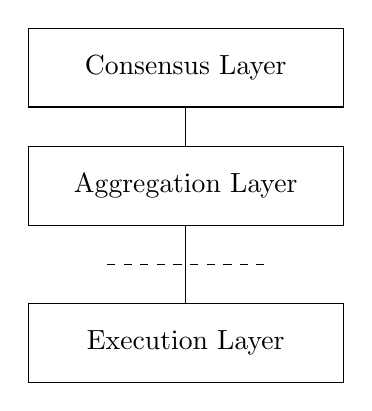
\begin{tikzpicture}
            \draw (0,0) rectangle (4,1) node[midway] {Consensus Layer};
            \draw (2,0) -- (2,-0.5);
            \draw (0,-1.5) rectangle (4,-0.5) node[midway] {Aggregation Layer};
            \draw[dashed] (1,-2) -- (3,-2);
            \draw (2,-1.5) -- (2,-2.5);
            \draw (0,-3.5) rectangle (4,-2.5) node[midway] {Execution Layer};
        \end{tikzpicture}
    \caption{Layered architecture of the Unicity Network.}\label{fig:layers}
\end{figure}


\subsection{Consensus Layer}
Decentralization is achieved by a Proof-of-Work (PoW) blockchain instance which manages consensus, including the validator selection for the BFT finality gadget, implementing the native token, executing the tokenomics plan, and handling the validator incentives. PoW is specifically robust during the bootstrapping of a decentralized system: when the number of validators fluctuates, the financial value of tokens is low, and token distribution is relatively concentrated. PoW shows great liveness properties. At the same time, PoW chains do not provide fast and deterministic finality: many blocks of confirmations are needed to achieve a reasonable level of certainty. In Unicity, this is mitigated by including a BFT ``finality gadget'' which runs rather fast, and the finality of transactions below is defined by the consensus of the BFT cluster.

The PoW layer provides permissionlessness, a core property of decentralized blockchains. Any validator can actively participate in mining, and blocks are chosen based on the longest-chain rule. By selecting a PoW mining puzzle that is resistant to acceleration by GPUs and ASICs (specifically: RandomX~\cite{randomx}), we aim to further democratize the participation in the network.

PoW chains encounter rollbacks (``reorgs'') when alternative chains with a greater cumulative PoW work emerge. Limiting the maximum length of alternative chains creates the risk of involuntary forking---both alternative chains may be too long for a rollback. This risk is specifically mitigated by a finality gadget. On the other hand, PoW chains are extremely robust. If any number of validators leave or join the network, the chain continues to grow, and the block rate eventually adjusts to the new total mining power. In short, PoW trades liveness for safety.

The purpose of BFT consensus layer is twofold: 1) to provide deterministic (one-block) finality for the layers below, and 2) to achieve a fast and predictable block rate. BFT consensus trades liveness for safety: it is more fragile, as its liveness depends on a supermajority (e.g., two thirds) of validators being online and cooperative at any moment.

The usual way to achieve \emph{permissionless} BFT consensus is to use a Proof-of-Stake (PoS) setup. This can be delicate, especially during the launch of a blockchain protocol: there are known weaknesses like ``nothing at stake attack'', and risk of centralization. PoW-based protocols (and longest-chain-rule protocols in general) are more robust and well-suited for achieving a wide initial token distribution and establishing token value for effective decentralization.

By combining a PoW chain with a BFT consensus layer, Unicity leverages the desirable properties of both mechanisms. The PoW chain provides decentralization, robustness, and high security for the base currency, while the BFT layer provides fast, deterministic finality for the Aggregation Layer.

In Unicity, the BFT layer operates at a much higher block rate than the PoW chain. Validators for the BFT Consensus Layer are selected infrequently from a pool of recent, high-performing PoW miners, based on a deterministic algorithm and PoW chain content; anyone can execute the algorithm to verify the selection. PoW validators may also delegate their BFT layer validation rights.

Consensus Layer validators receive their block rewards at the ends of epochs. It is possible to increase economic security by implementing slashing based on withheld PoW and Consensus Layer block rewards.

\subsubsection{Consensus Roadmap}\label{sec:consensus-roadmap}

The introduction of economic security mechanisms is a logical step toward evolving the Consensus Layer into a full Proof-of-Stake (PoS) system, once the chain is stable and token distribution reasonably diversified. A PoS system would provide stronger economic security for the BFT nodes while being more energy-efficient and environmentally responsible than PoW mining.

The switch to PoS includes the following steps: 1) introducing the staking mechanism to create economic security for the BFT layer, 2) alternative ledger for the native token securing and decentralizing the system, and executing the tokenomics plan there, 3) selecting BFT validators based on the stake, 4) adjusting incentives (block rewards, optional slashing), 5) migrating the token balances, and 5) sunsetting the PoW chain.

\subsection{Proof Aggregation Layer}

The Aggregation Layer implements a global, append-only key-value store that immutably records every spent token state. More specifically, it provides the following services: 1) recording of key-value tuples where the key identifies a token state and value is recording some meta-data, 2) returning inclusion proofs of keys, 3) returning non-inclusion proofs of keys not present in the store.

The Aggregation Layer periodically has its state authenticator certified by the Consensus Layer.

\begin{figure*}[!t]
    \centering
    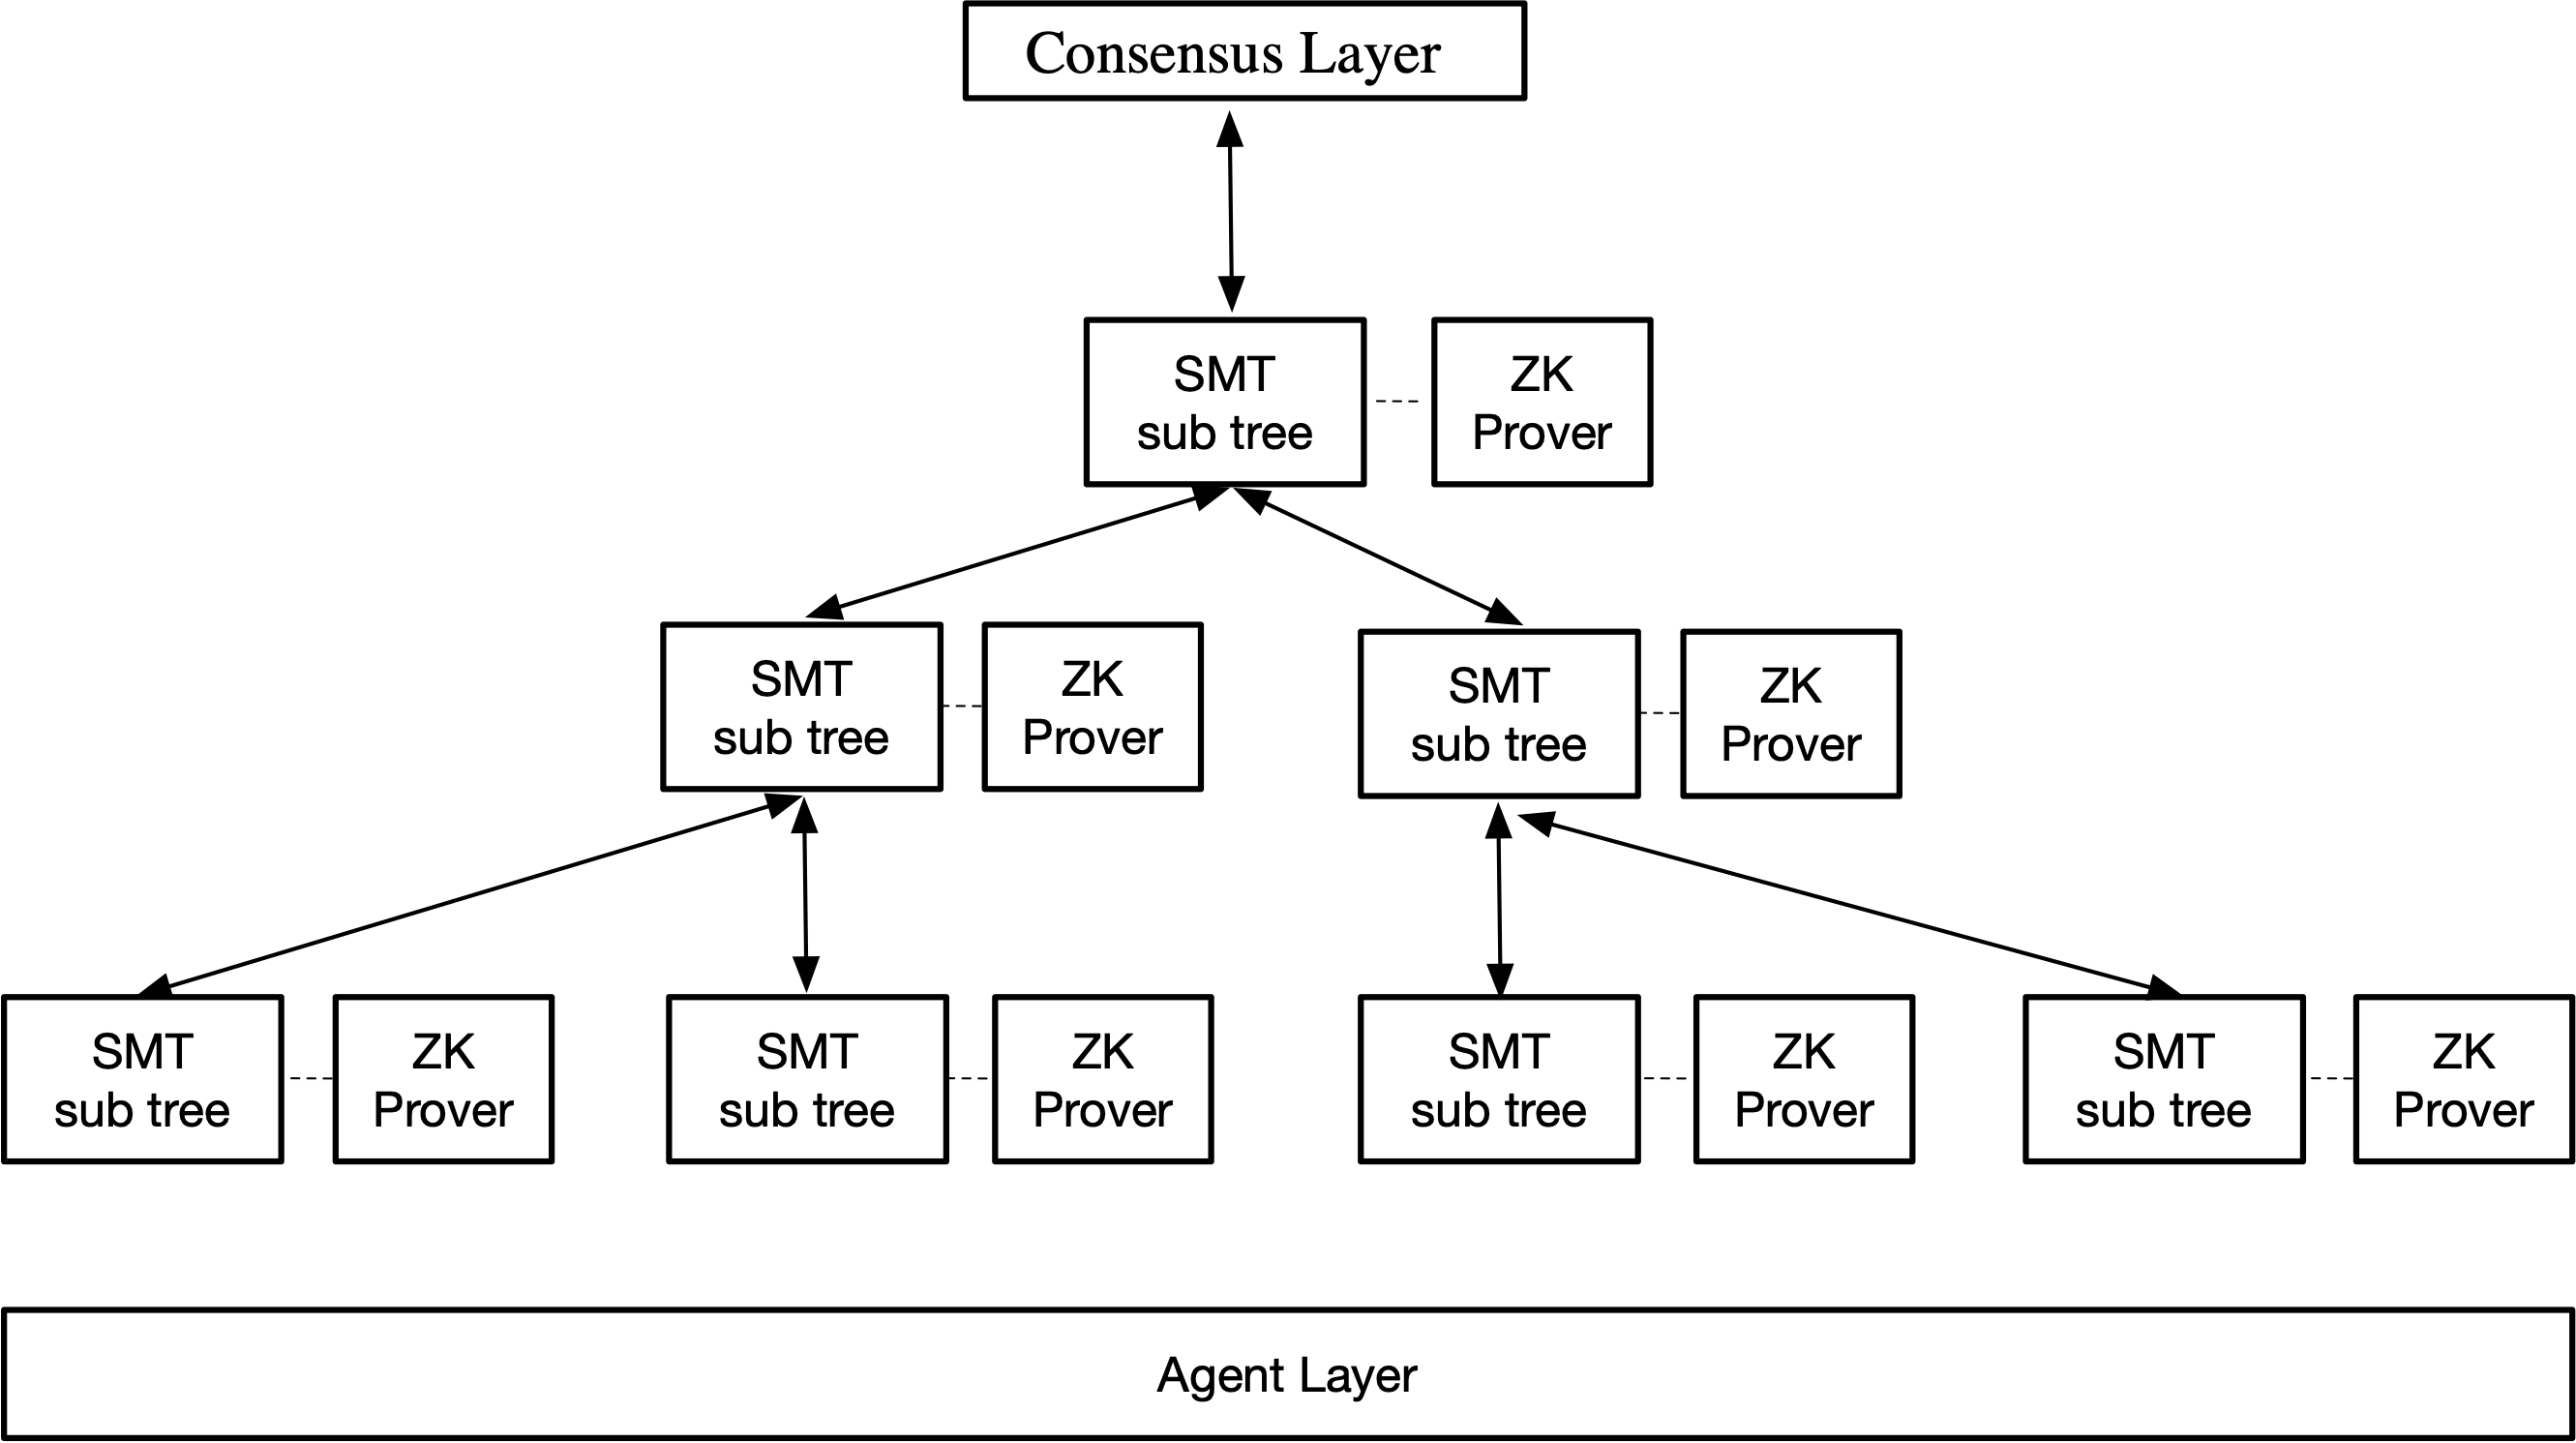
\includegraphics[width=.7\textwidth]{pic/layers}
    \caption{Sharded architecture of the Aggregation Layer.}\label{fig:sharding}
\end{figure*}

The Aggregation layer is sharded based on keyspace slices and can be made hierarchical, as shown in Figure~\ref{fig:sharding}.

\emph{Proof of non-deletion}: Once a key is set, it has to remain there forever. Every state change of the Aggregation Layer (or a slice thereof) is accompanied by a cryptographic proof establishing that pre-existing keys have not been removed or their values altered, only new keys were added. The size of this proof is logarithmic with respect to the tree's capacity and linear with respect to the size of the inclusion batch. This can be reduced to a constant size using a SNARK. Assuming correct validation of the non-deletion proof and chaining of the Aggregation Layer's state roots by the Consensus Layer, the Aggregation Layer can be considered trustless.


\subsection{Execution Layer}

The Execution Layer, also known as the Agent Layer, is responsible for executing transactions and other business logic, using the services of the Aggregation Layer and Unicity in general.


\section{Security Model of the Aggregation Layer}

The Aggregation Layer implements a distributed, authenticated, append-only dictionary data structure.
It authenticates incoming state transfer certification requests by verifying that the sender possesses the private key corresponding to the public key that identifies the current token owner. The specific authentication protocol is beyond the scope of this paper.

\begin{definition}[Consistency]
An append-only accumulator operates in batches $B = (k_1, k_2, \ldots, k_j)$, accepting new keys. The append-only accumulator is \emph{consistent}, if 1) during the insertion of a batch of updates, no existing element was deleted or modified; 2) it is possible to generate inclusion proofs $\pi^{\textsf{inc}}_{k \in \{B_1, \dots, B_i\}} = (v_k \leadsto r, c)$ for all previously inserted elements, but not for non-existent elements; 3) it is possible to generate non-inclusion proofs $\pi^{\overline{\textsf {inc}}}_{k \notin \{B_1, \dots, B_i\}} = (\varnothing_k \leadsto r, c)$ for all elements not so far inserted to the accumulator, and not for those already inserted.
\label{def:append-only-accumulator}
\end{definition}

When instantiated as a Sparse Merkle Tree (SMT), then $v_k \leadsto r$ is the hash chain from the value at $k$-th position to root $c$, and $\varnothing_k \leadsto r$ denotes the hash chain from the ``empty'' value at $k$-th position to root $c$.

After each batch of additions, the new root of the Aggregation Layer's SMT is certified by the BFT finality gadget, ensuring its uniqueness and immutability. This provides a secure trust anchor for all consistency, inclusion, and non-inclusion proofs. The idealized Consensus Layer is modeled as Algorithm~\ref{alg:consensuslayer}.


\begin{figure}[!htbp]
    \centering
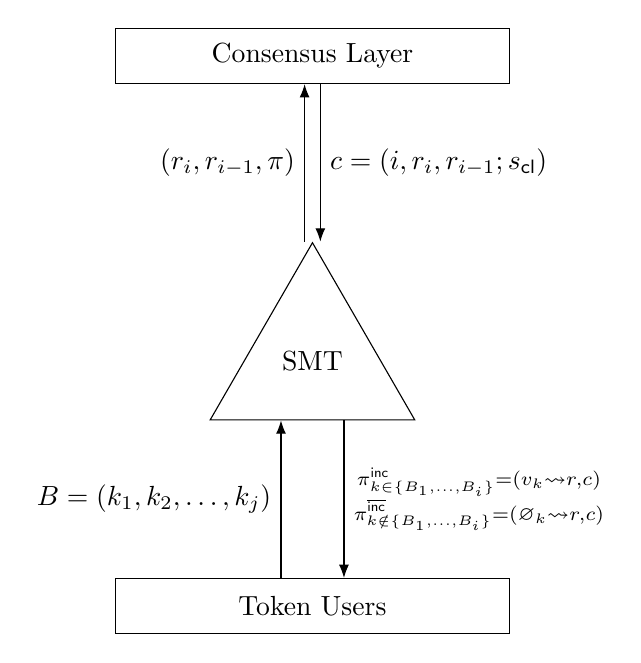
\begin{tikzpicture}[node distance=2cm and 2cm]

    % Nodes
    \node[block] (consensus) {Consensus Layer};
    \node[triangle, below=of consensus] (triangle) {SMT};
    \node[block, below=of triangle] (users) {Token Users};

    % Arrows
    \draw[arrow] ([xshift=-0.1cm]triangle.north) -- ++(0,1) node[labelstyle, left] {$(r_i, r_{i-1}, \pi)$} -- ([xshift=-0.1cm]consensus.south);
    \draw[arrow] ([xshift=0.1cm]consensus.south) -- node[labelstyle, right] {$c = (i, r_i, r_{i-1}; s_{\textsf{cl}})$} ([xshift=0.1cm]triangle.north);
    \draw[arrow] ([xshift=-0.4cm]users.north) -- node[labelstyle, left] {$B = (k_1, k_2, \ldots, k_j)$} ([xshift=-0.4cm]triangle.south);
    \draw[arrow] ([xshift=0.4cm]triangle.south) -- ++(0,-1) node[labelstyle, right] {
            $\substack{
                \pi^{\textsf{inc}}_{k \in \{B_1, \dots, B_i\}} = (v_k \leadsto r, c) \\
                \pi^{\overline{\textsf {inc}}}_{k \notin \{B_1, \dots, B_i\}} = (\varnothing_k \leadsto r, c)
            }$
            } -- ([xshift=0.4cm]users.north);

\end{tikzpicture}
    \caption{Security model of the Aggregation Layer.}\label{fig:model}
\end{figure}

For efficiency reasons client requests are processed in batches; the tree is re-calculated and the tree root is certified when a batch is closed. A batch of client requests is denoted as $B_i$. At the end of each batch, the Aggregation Layer produces its summary root hash $r_i$ and sends it to the Consensus Layer for certification. A certification request $(r_i, r_{i-1}, \pi)$ includes: 1) the previous state root hash, 2) the new state root hash, 3) a consistency proof of the changes made during the batch, and 4) an authenticator that identifies the operator.

The Consensus Layer certifies the request only if it uniquely \textit{extends} a previously certified state root and the consistency proof is valid. It returns a certificate $c = (i, r_i, r_{i-1}; s_{\textsf{cl}})$, where $s_{\textsf{cl}}$ is a signature from the Consensus Layer (e.g., a threshold signature from the consensus nodes or a proof of inclusion in a finalized block).

Each state can be extended only once, which prevents forks within the Aggregation Layer. Each subsequent round extends the most recently certified state.
We model the Consensus Layer as an oracle, as shown in Algorithm~\ref{alg:consensuslayer}.

\begin{algorithm}[tbh]
  \caption{Consensus Layer modeled as an oracle}\label{alg:consensuslayer}
  \begin{algorithmic}[0]
    \Function{Initialize}{\null}
        \State $r_- \gets \bot$
        \State $i \gets 0$
    \EndFunction
    \Function{CertificationRequest}{$r_i, r_{i-1}, \pi$}
        \If {$(r_{i-1} \ne  r_-) \lor \lnot\Call{valid}{\pi, r_i, r_{i-1}}$}
            \State \Return $\bot$
        \EndIf
        \State $r_- \gets r_i$
        \State $i \gets i+1$
        \State $s_{\textsf{cl}} \gets \textsf{sig}_\textsf{cl}(i, r_i, r_{i-1})$
        \State \Return $c = (i, r_i, r_{i-1}; s_{\textsf{cl}})$
    \EndFunction
  \end{algorithmic}
\end{algorithm}


The SMT provides users with inclusion and non-inclusion proofs. Each proof is anchored to a state root certified by the Consensus Layer.

The Consensus Layer must guarantee data availability. If recent state roots were lost, it would become impossible to reject duplicate state transition requests, potentially allowing malicious actors to double-spend against an old, un-extendable state. The Aggregation Layer itself does not require an internal consensus mechanism; protocols like Raft could be used for replication and coordination among its redundant nodes. The decentralized consensus is provided by the external Consensus Layer.

If each state transition is accompanied by a cryptographic proof of non-deletion (see Section~\ref{sec:consistency-proof}), the Aggregation Layer can be considered trustless.


\subsection{``Maximalist'' Security Assumptions}

In this model, we assume that users are capable of validating all aspects of system operation that are relevant to their own assets. This level of trustlessness is close to the strong guarantees introduced by Bitcoin~\cite{bitcoin}, where each ``client'' functions as a full validator, starting from downloading and verifying the blockchain from the genesis block.

The Root of Trust is the PoW blockchain. A maximalist user maintains a full node of this chain. This is relatively lightweight, as the ``utility'' transactions are executed at the Execution Layer. Upon receiving a token, the user must be able to efficiently verify the following:

\begin{enumerate}[nosep]
    \item The token is valid (as elaborated elsewhere),
    \item The Aggregation Layer has not forked,
    \item The Aggregation Layer has not certified conflicting states of the same token.
\end{enumerate}

The second point is addressed by validating a unique state root snapshot embedded in the PoW block header. Since the cumulative state snapshot appears with a delay, the block can only be considered final after a snapshot publishing and block confirmation period; hence, maximalist verification is not instantaneous.

The third point is addressed by auditing the operation of the Aggregation Layer—specifically, ensuring that no Inclusion Proofs have been generated for the token that are not reflected in its recorded history. To achieve this, all non-deletion proofs from the token's genesis up to its current state must be validated. This is made efficient through the use of recursive zero-knowledge proofs (ZKPs), which show that each round’s non-deletion proof is valid and that no rounds were skipped from verification. These recursive proofs are generated periodically and are made available with some latency.

\subsection{Practical Security Assumptions}

If we relax the model by assuming that a majority of BFT consensus nodes exhibit economically rational behavior and do not collude maliciously with the Aggregation Layer, the user can enjoy significantly more practical operational parameters. BFT layer forking (case 2 above) or certifying conflicting states (case 3 above) produces strong cryptographic evidence which is processed out of the critical path of serving users.

In this scenario, a transaction is finalized, and an inclusion proof is returned within a few seconds, allowing the transaction to be independently verified—without consulting external data\footnote{Previously obtained Root of Trust is used to validate future transactions}—within the same timeframe.

The Root of Trust is the set of epoch change records of the BFT consensus layer. These records grow slowly (few aggregated signatures per week). When transitioning to proof-of-stake (PoS) consensus (see Section~\ref{sec:consensus-roadmap}), the Root of Trust remains the same.


\section{Non-deletion Proof}
\label{sec:consistency-proof}

A non-deletion proof is a cryptographic construction that validates one round of operation of  the append-only accumulator.

We have the $i$-th batch of insertions $B_i = (k_1, k_2, \dots, k_j)$, where $k$ is an inserted item; all insertions are applied within a single operational round. The root hash before the round is $r_{i-1}$, and after the round is $r_i$. The accumulator is implemented as a Sparse Merkle Tree (SMT).

The non-deletion proof generation for batch $B_i$ works as follows:

\begin{enumerate}
    \item The new leaves in batch $B_i$ are inserted into the SMT.
    \item For each newly inserted leaf, the sibling nodes on the path from the leaf to the root are collected. Siblings present or computable from other leaves in the batch are discarded. Siblings can be further organized by dividing them into layers, for more efficient verification. We denote the set as $\pi_i$.
    \item Record $(B_i, r_{i-1}, r_i, \pi_i)$.
\end{enumerate}

Proof verification works as follows:

\begin{enumerate}
    \item Verify the authenticity of the state roots $r_{i-1}$ and $r_i$ (e.g., by checking their certification by the Consensus Layer).
    \item Build an incomplete SMT tree: for each item in $B_i$, insert the value of an empty leaf at the appropriate position.
    \item All non-computable siblings needed to compute the root are available in $\pi_i$. Compute the root, compare with $r_{i-1}$; if not equal then the proof is not valid.
    \item Build again an incomplete SMT tree; for each item in $B_i$, insert the value of the key into the appropriate position.
    \item Compute the root based on siblings in $\pi_i$. If the root is not equal to $r_i$ then the proof is not valid.
    \item The proof is valid if the checks above passed.
\end{enumerate}

A valid proof demonstrates that, given authentic roots $r_{i-1}$ and $r_i$, the keys in $B_i$ corresponded to empty leaves prior to the update, and that after the update, the values in $B_i$ were recorded at the positions defined by their respective keys, and there were no other changes.

Complete verification algorithm is presented as Algorithm~\ref{alg:verifynondeletion}. Note that there are several assumptions: that the batch is sorted by keys; and the proof is an array of arrays of tuples, outer array divides siblings into depth layers and inner array is sorted by keys (first element of tuple).

Due to the sparseness of the SMT we can further improve the encoding, for example, instead of checking if a node's sibling is the next item in layer's nodes or the next item in proof array or empty element otherwise, we just record a number--how many of the next siblings are empty elements (frequent close to the leaves when SMT is sparsely populated); and same with siblings (frequent close to the root).

\begin{algorithm}[htb]
  \caption{Verification of non-deletion proof}\label{alg:verifynondeletion}
  \begin{algorithmic}[0]
    \Function{VerifyNonDeletion}{$\pi, r_{i-1}, r_i, P$}
      \State   \Comment{Proof $\pi$ is a by-layer array of ...}
      \State   \Comment{... sorted arrays of k-v tuples}
      \State   \Comment{Insertion batch $P$ is ...}
      \State   \Comment{... sorted array of k-v tuples}
      \State $p_\varnothing \gets \{(k, \varnothing) \mid (k, v) \in P\}$ \Comment{Empty leaves}
      \State $r_\varnothing \gets$ \Call{ComputeForest}{$\pi, p_\varnothing$}
      \State \textbf{assert} $r_\varnothing = r_{i-1}$
      \State \Comment{Same with batch's leaves populated}
      \State $r_B \gets$ \Call{ComputeForest}{$\pi, P$}
      \State \textbf{assert} $r_B = r_i$
      \State \Return $1$ \Comment{Success}
    \EndFunction

    \Function{ComputeForest}{$\pi, p$}
      \For{$\ell \in \text{tree\_depth}$}
        \State $p' \gets [\,]$     \Comment{computed nodes of parent layer}
        \State $m \gets 0 ; n \gets 0$  \Comment{indices}
        \While{$m < |p|$}
          \State $(k, v) \gets p[m]$
          \State $k_p \gets \lfloor k / 2 \rfloor$ \Comment{Parent key}
          \State $\text{is\_right} \gets k \bmod 2$
          \State $k_s \gets 2k_p + (1 - \text{is\_right})$ \Comment{Sibling key}
          \If{$\lnot \text{is\_right} \land |p| > m+1 \land p[m+1].k = k_s$\\ \hskip 4em}
                \Comment{Right sibling is next}
            \State $v_s \gets p[m+1].v$
            \State $m \gets m + 1$       \Comment{Jump over}
             % j < len(lproof) and lproof[j][0] == sibling
          \ElsIf{$|\pi[\ell]| > n \land \pi[\ell][n].k = k_s$}
            \State $v_s \gets \pi[\ell][n].k$
            \State $n \gets n + 1$
          \Else
            \State $v_s \gets \varnothing$
          \EndIf
          \State $v_p \gets h(v_s, v)$ \textbf{if} is\_right \textbf{else} $h(v, v_s)$
          \State $p' \gets p' \| (k_p, v_p)$
          \State $m \gets m + 1$
        \EndWhile
        \State $p \gets p'$
      \EndFor
      \State \textbf{assert} $|p| = 1$ \Comment{One root!}
      \State \Return $p[0].v$ \Comment{Value of the root}
    \EndFunction
  \end{algorithmic}
\end{algorithm}


\section{(ZK)-SNARKs}

By using an appropriate cryptographic SNARK system, the size of the non-deletion proof can be reduced to a constant.

The statement to be proven in zero-knowledge is the correct execution of the non-deletion proof verification algorithm described in the previous section. The public inputs to the proof (the instance) are the pre- and post-update roots $(r_{i-1}, r_i)$. The private input (the witness) $\omega$ is the insertion batch $B_i$ and the set of sibling nodes (proof) $\pi_i$. While ZK-SNARKs can hide the witness, this zero-knowledge property is not a requirement for our use case; we are primarily interested in the proof's succinctness.

In an experiment~\cite{snark}, the statement is implemented as a constraint system $R$ using the CIRCOM domain-specific language. The witness is generated based on $\pi_i$ and $B_i$, and is supplemented by control wires that define how individual hashing blocks in the circuit are connected to the previous layer and to the inputs. If all constraints are satisfied, the proof is valid.

The proving system used is Groth16~\cite{cryptoeprint:2016/260}, which is known for its small proof size. The proving time depends on the depth of the SMT (logarithmic in its capacity) and the maximum size of the insertion batch. Importantly, the proving effort does not depend on the total capacity of the SMT, enabling fairly large instantiations.

When the Consensus Layer verifies these succinct proofs, the Aggregation Layer operates trustlessly. However, certain redundancy is still required to ensure data availability of the SMT itself.


\section{Circuit-Based SNARK Definition}

Due to the limited expressivity of an arithmetic circuit (e.g., no data-dependent loops or real branching), the entire computation flow must be fixed at circuit-creation time. It is therefore helpful to pre-process the inputs to create a fixed execution trace.

This pre-processing generates a ``wiring'' signal, which is supplied as part of the witness. This signal dictates the data flow between the hashing units within the circuit.

To preprocess the proof:

\begin{enumerate}
    \item The hash forest, which includes the proof's sibling nodes and the new batch leaves, is flattened.
    \item The nodes are sorted first by layer (from leaves to root) and then lexicographically within each layer.
    \item A wiring signal is generated to control the multiplexers (MUXes) at the input of each hashing unit in the circuit.
\end{enumerate}

Let the maximum batch size be $k_{max}$ and the SMT depth be $d$. Since the arithmetic circuit is static, it must be designed to accommodate the maximum possible batch size, $k_{max}$.

The circuit has two halves, both controlled by the same wiring signal. It is critical to security that the control signal and the proof are the same for both halves. The first half of the circuit computes the pre-update root by treating all leaves in the insertion batch as zero (the value of empty leaf). The second half computes the post-update root using the actual values from the batch. The number of hashing units in each half of the circuit is approximately $O(k_{max} \cdot d)$.

Each hashing unit takes its inputs either from the outputs of the previous layer's units or from the set of sibling nodes provided in the proof. The pre-processing step encodes the positions of batch and proof elements into these control signals, which are then supplied as part of the witness.

\begin{figure*}[!t]
    \centering
    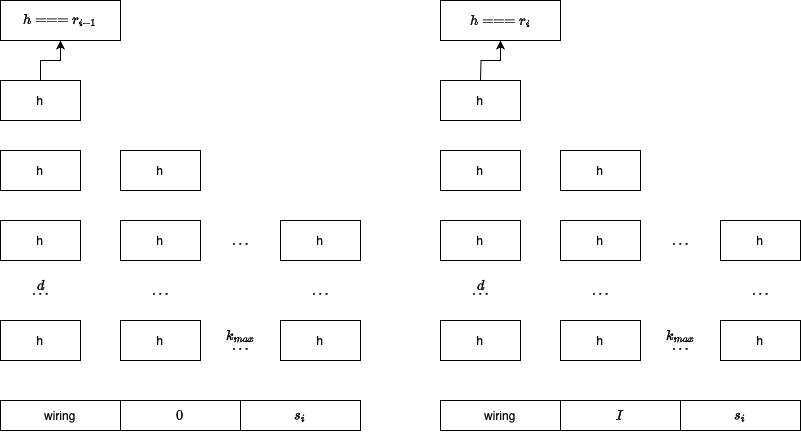
\includegraphics[width=0.9\textwidth]{pic/smt-circuit.drawio}
    \caption{Circuit structure.}\label{fi:smt-circuit}
\end{figure*}

Each hashing cell in the circuit, as depicted in Figure~\ref{fi:smt-circuit-cell}, is a template consisting of two input multiplexers and one 2-to-1 compressing hash function.

\begin{figure}[t]
    \centering
    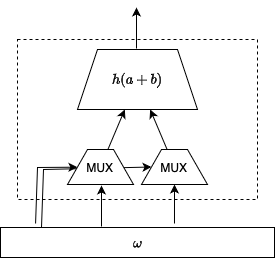
\includegraphics[width=.6\columnwidth]{pic/smt-circuit-cell.drawio}
    \caption{One hashing cell of the circuit.}\label{fi:smt-circuit-cell}
\end{figure}


The MUX inputs for the leaf layer of the first half are connected to a vector containing:
\begin{itemize}
    \item The ``empty'' leaf value ($0$).
    \item All new leaves in the batch, which are mapped to `empty' ($0$).
    \item The ``proof'' or sibling hashes ($\pi_i$).
\end{itemize}

The MUX inputs for the leaf layer of the second half are connected to a vector containing:
\begin{itemize}
    \item The ``empty'' leaf value ($0$).
    \item The batch of new leaves ($I$).
    \item The identical ``proof'' or sibling hashes ($\pi_i$).
\end{itemize}

The MUXes for internal layers are connected to a vector containing:
\begin{itemize}
    \item The ``empty'' leaf value ($0$).
    \item Output hashes from the previous layer's cells.
    \item The ``proof'' or sibling hashes ($\pi_i$).
\end{itemize}

Both halves' MUXes are controlled by the same wiring signal.

\subsection{Performance Indication}

Initial benchmarks on a consumer laptop (Apple M1) using the Poseidon hash function indicate a proving throughput of up to $25$ transactions per second.


\section{Execution Trace-Based STARK}

An alternative to a bespoke arithmetic circuit is to use a general-purpose zero-knowledge virtual machine (zkVM). In this approach, the verification logic is written as a traditional imperative program (e.g., in Rust). The zkVM then generates a proof of correct execution for that program.

We have implemented the non-deletion proof verification algorithm as a Rust program~\cite{stark} to be proved by the SP1 zkVM~\cite{sp1}. As a commitment to the ``right'' program we use a prover key, generated during program setup. Its contents are: a commitment to the preprocessed traces, the starting Program Counter register, the starting global digest of the program, after incorporating the initial memory; the chip information, the chip ordering; and prover configuration.

For verification, we obtain the prover key hash and authenticate it off-band.

%\begin{sloppypar}
After verifying the proof (\lstinline|client.verify(&proof, &vk)|), we can be sure that \lstinline|proof: SP1ProofWithPublicValues| is valid. The proof data structure embeds its validated ``instance'', or public parameters. Based on these parameters we check that indeed, the right thing was executed. In our case the instance is defined by the old root hash and the new root hash, which must be authenticated independently (i.e., using the certificate from Consensus Layer).
%\end{sloppypar}

The privacy of the witness (the zero-knowledge property) is not a requirement for this application. The primary goal is to achieve computational integrity and succinctness. Therefore, while the underlying technology is often referred to as ``ZK'', we are using it as a Scalable Transparent ARgument of Knowledge (STARK).

\subsection{zkVM Performance}

On a 10-core Apple M1 CPU, proving a 500-transaction batch using SHA-256 within the SP1 zkVM takes approximately 5 minutes. However, the SP1 framework is robust and designed for scalability, supporting distributed prover networks, industrial-grade GPUs, proof chunking and recursion, and other advanced features to tackle larger problems with brute force.


\subsection{Optimization Ideas}

The ZK proving performance is dominated by the cryptographic hashing primitive used by the program.

At the time of writing, the SP1 zkVM\footnote{\url{https://docs.succinct.xyz/docs/sp1/introduction}} offers precompiles for standard hash functions like SHA-256, which accelerates their execution compared to a direct RISC-V implementation. The use of these precompiles (also known as coprocessors or chips) can be observed in the prover's output, which details the number of calls to each specialized circuit (e.g., \lstinline|SHA_EXTEND|, \lstinline|SHA_COMPRESS|). However, even with acceleration, proving SHA-256 is computationally expensive.

A possible optimization is to use ``ZK-friendly'' hash functions. These functions are highly efficient when implemented directly in arithmetic circuits, where there is direct access to the native field elements. Their performance advantage in a RISC-V zkVM is more nuanced, as there is an overhead in translating between the VM's 32-bit integer registers and the underlying finite field elements as used by the prover. Operations like range-checking, which are necessary to prevent overflows, are expensive in ZK. There are attempts to create precompiles for ZK-friendly hash functions\footnote{\url{https://github.com/Okm165/sp1-poseidon2/pull/8}}, with limited real-world effect.


\subsection{More on ZK and Hash Functions}

Standardized cryptographic hash algorithms like SHA-2 were optimized mostly for minimal physical chip area, a design choice driven by NIST. Others, like the Blake family, were designed for fast execution on CPUs. They all include numerous bitwise operations (e.g., rotations, XOR) that are silicon logic-native but are notoriously inefficient to prove in ZK. Proving such operations is expensive, because a full field element (e.g., a 254-bit value on the BN254 curve) must be used to represent a single bit.\footnote{See e.g. \url{https://github.com/iden3/circomlib/blob/master/circuits/sha256/sha256.circom}} ZK provers are most efficient with arithmetic operations native to the underlying finite field, such as addition and multiplication (and lookups on some ZK stacks). Other operations must be implemented indirectly.

There are some newer cryptographic hash functions specifically designed for ZK efficiency in mind. Functions like Poseidon and Poseidon2 are gaining acceptance but are still relatively new. Some are better on large fields (e.g., Reinforced Concrete), some on smaller (e.g., Monolith) and depending on the proof system's lookup table support. Even newer and exhibiting even higher performance examples are Griffin, Anemoi. Some, like GMiMC, are offering a compromise with better silicon CPU performance.

A key advantage of these hashes is that they operate directly on field elements, avoiding the costly translation from integer representations. The security level is defined by the underlying field and instantiation parameters. While some VMs, like the Cairo VM used by Starknet, provide direct access to field elements, they are often highly specialized for particular use cases, such as L2 rollups.


\subsection{Performance Roadmap}

The overall approach is sound: the proving time depends on the size of the addition batch, and notably, it does not have linear relationship to the total capacity of the data structure. The verification algorithm is tight.

To overcome the performance bottleneck, a ZK-friendly hash function is essential. The ideal proving framework would provide direct access to the native field elements of its arithmetization layer, a feature not typically available in general-purpose zkVMs. Execution trace generation must be highly efficient (a criterion that excludes older frameworks like Cairo~0). The prover itself must be fast. State-of-the-art uses small prime fields (e.g., BabyBear, Mersenne-31) and FRI-based polynomial commitment schemes, like Circle-STARKs~\cite{cryptoeprint:2024/278}. Promising implementations are Plonky3\footnote{\url{https://github.com/Plonky3/Plonky3}} and STwo\footnote{\url{https://github.com/starkware-libs/stwo}}. Considering the need for maturity, modularity, and an open-source license, Plonky3 emerges as the strongest option.

To utilize the Plonky3 framework, the verification logic must be implemented as a custom AIR circuit (Algebraic Intermediate Representation) rather than a general-purpose program.

\subsection{Custom AIR Circuit}
\label{sec:custom-air-circuit}

Extrapolating from benchmarks of similar computations~\footnote{Experiment with iterative hashing and a hash-based signature scheme \url{https://github.com/han0110/hash-sig-agg/}} using the Plonky3 framework, Poseidon2 hash function, and a small finite field, the projected performance of such a stack on a 10-core CPU is approximately 10\,000\;tx/s. The parameter ``blowup factor'' is $2^1$, resulting in a 1.7\;MB proof. A more conservative configuration with a blowup factor of $2^3$ would yield approximately 2500\;tx/s with a 0.7\;MB proof and higher memory requirements for the prover.

These figures indicate that operating very large-scale Aggregation Layer in a trustless manner is economically feasible.

We note that the Poseidon family of hash functions is relatively new and has undergone less cryptographic analysis than traditional hash functions like the SHA-2 or SHA-3 families. However, among the new class of ZK-friendly arithmetic hash functions, Poseidon has undergone the most public scrutiny and can be tentatively considered secure for this type of application. It offers an estimated 50$\times$ improvement in proving performance compared to efficient standard hash function like Blake3.

\section{Summary}

Zero-knowledge proof systems offer a powerful method for creating succinct proofs of performing some computation, in our case, checking consistency proofs of a distributed cryptographic data structure. For use cases with small changesets, a simple hash-based proof, whose size is linear in the batch size, is optimal. However, as batch sizes increase and bandwidth becomes a constraint, the constant or near-constant size proofs generated by ZK systems become more advantageous.

Different proof systems offer different trade-offs. The properties are: proving effort, necessity of trusted setup, generality of trusted setup, interactivity, proof recursion-friendliness, and of course properties like availability of tooling, maturity, trustworthiness. Some, like STARKs, are relatively fast to prove but have fairly large proofs; and avoid undesirable properties such as trusted setup. Others, like Groth16, produce small proofs but require more proving effort and a circuit-specific trusted setup. For more complex applications, hybrid approaches and proof recursion can be employed. Figure~\ref{fig:comp} illustrates the proof size trade-off.

\begin{figure}[!htbp]
    \centering
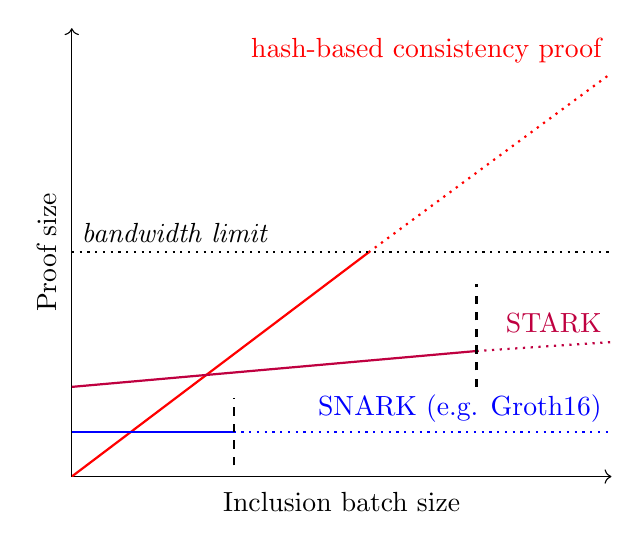
\begin{tikzpicture}
\begin{axis}[
axis lines = left,
axis line style={->},
xlabel = {Inclusion batch size},
ylabel = {Proof size},
xmin=0, xmax=10,
ymin=0, ymax=10,
xtick=\empty,
ytick=\empty,
]
\addplot [red, thick, smooth] coordinates {(0,0)  (5.5, 5)};
\addplot [red, thick, dotted] coordinates {(5.5, 5)  (10,9)};
\node [red, above left] at (axis cs:10,9) {hash-based  consistency proof};

\addplot [purple, thick, smooth] coordinates {(0,2) (7.5,2.8)};
\addplot [purple, thick, dotted] coordinates {(7.5,2.8) (10,3)};
\node [purple, above left] at (axis cs:10,3) {STARK};

\addplot [blue, thick, smooth] coordinates {(0,1) (3,1)};
\addplot [blue, thick, dotted] coordinates {(3,1) (10,1)};
\node [blue, above left] at (axis cs:10,1) {SNARK (e.g. Groth16)};

% perf limits
\addplot [dotted, thick] coordinates {(0,5) (10,5)};
\node [above right] at (axis cs:0,5) {\it bandwidth limit};

\addplot [dashed, thick] coordinates {(3, 0.25) (3, 1.75)}; % snark
\addplot [dashed, thick] coordinates {(7.5, 2) (7.5, 4.3)};   % stark

\end{axis}
\end{tikzpicture}
    \caption{Proof size vs. use of ZK compression. Dotted line is bandwidth limit, dashed line is compute limit (ZK scheme specific). Not to scale.}\label{fig:comp}
\end{figure}

\bibliographystyle{plain}
\bibliography{aggregation-layer}


\end{document}